\chapter{Models in Django}
\section{Introduction to Django Models}
\paragraph{} \textbf{Models and Databases in Django:}\\
A model is the single, definitive source of data about your data. It contains the essential fields and behaviors of the
data you're storing. Generally, each model maps to a single database table.
\subsection{Models}
A model is the single, definitive source of information about your data. It contains the essential fields and behaviors
of the data you're storing. Generally, each model maps to a single database table.
\\ \\ Basic concepts:
\begin{itemize}
	\item Each model is a Python class that subclasses \textbf{django.db.models.Model}.
	\item Each attribute of the model represents a database field.
	\item With all of this, Django gives you an automatically-generated database-access API.
\end{itemize}
 Using Models:\\
When you add new apps to INSTALLED\_APPS, be sure to run \textbf{./manage.py migrate},optionally making migrations for them first with \textbf{./manage.py makemigrations}.

\newpage
\subsection{Model Fields}
\subsubsection{Introduction}
Each field in your model should be an instance of the appropriate Field class. Django uses the field class types to
determine a few things:
\begin{itemize}
	\item The column type, which tells the database what kind of data to store (e.g. INTEGER, VARCHAR, TEXT).
	\item The default HTML widget to use when rendering a form field (e.g. <input type="text">, <select>).
	\item The minimal validation requirements, used in Django's admin and in automatically-generated forms.
\end{itemize}
\subsubsection{Field Options}
A set of common arguments available to all field types. All are optional. Most oftenly used field options are:
\begin{itemize}
	\item \textbf{null} If True, Django will store empty values as NULL in the database. Default is False.
	\item \textbf{blank} If True, the field is allowed to be blank. Default is False.
	\item \textbf{choices} An iterable of 2-tuples to use as choices for this field. If this is given, the default form widget will be a select box instead of the standard text field and will limit choices to the choices given.
	\begin{lstlisting}[language=python,numbers=none]
	 
	 YEAR_IN_SCHOOL_CHOICES = [
	 ('FR', 'Freshman'),
	 ('SO', 'Sophomore'),
	 ('JR', 'Junior'),
	 ('SR', 'Senior'),
	 ('GR', 'Graduate'),
	 ]
	\end{lstlisting}
	\item \textbf{primary\_key} primary\_key If True, this field is the primary key for the model
\end{itemize}
\newpage
\subsection{Relationships}
Types of Django models relationships:
\begin{itemize}
	\item Many-to-one relationship.
	\item Many-to-Many relationship.
\end{itemize}
\subsubsection{Many-to-One relationship}
To define a many-to-one relationship, use \textbf{django.db.models.ForeignKey}. You use it just like any other Field type: by including it as a class attribute of your model.
\textbf{ForeignKey} requires a positional argument: the class to which the model is related.
\begin{lstlisting}[language=python,numbers=none]

from django.db import models
class Manufacturer(models.Model):
# ...
pass

class Car(models.Model):
manufacturer = models.ForeignKey(Manufacturer, on_delete=models.CASCADE)  
\end{lstlisting}

\subsubsection{Many-to-Many relationship}
To define a many-to-many relationship, use \textbf{ManyToManyField}. You use it just like any other Field type: by including it as a class attribute of your model.
\textbf{ManyToManyField} requires a positional argument: the class to which the model is related.
\begin{lstlisting}[language=python,numbers=none]
  from django.db import models
  class Topping(models.Model):
  # ...
  pass
  
  class Pizza(models.Model):
  # ...
  toppings = models.ManyToManyField(Topping)
\end{lstlisting}

\newpage

\section{Model instance reference}
\subsection{Creating objects}
To create a new instance of a model, just instantiate it like any other Python class:
\textbf{class Model(**kwargs)}.
Steps:
\begin{enumerate}
	\item Add a class method on model class:
	\begin{lstlisting}[language=python,numbers=none]
	from django.db import models
	
	class Book(models.Model):
	
		title = models.CharField(max_length=100)
		@classmethod
		def create(cls, title):
			book = cls(title=title)
			# do something with the book
			return book
		book = Book.create("Pride and Prejudice")
	\end{lstlisting}
	\item  Add a method on a custom manager (usually preferred):
	\begin{lstlisting}[language=python,numbers=none]
	class BookManager(models.Manager):
		def create_book(self, title):
			book = self.create(title=title)
			# do something with the book
			return book
	class Book(models.Model):
		title = models.CharField(max_length=100)
		objects = BookManager()
		book = Book.objects.create_book("Pride and Prejudice")
	\end{lstlisting}
\end{enumerate}
\subsection{Validating objects}
There are three steps involved in validating a model:
\begin{enumerate}
	\item Validate the model fields - \textbf{Model.clean\_fields()}.
	\item Validate the model as a whole - \textbf{Model.clean()}.
	\item Validate the field uniqueness - \textbf{Model.validate\_unique()}.
\end{enumerate}
\newpage
\subsection{Saving Model Object}
To save an object back to the database, call save():
\begin{lstlisting}[language=python,numbers=none]
Model.save(force_insert=False, force_update=False,using=DEFAULT_DB_ALIAS, update_fields=None)
\end{lstlisting}
\subsection{What happens when you save?}
\begin{enumerate}
	\item  \textbf{Emit a pre-save signal}- The \textbf{pre\_save} signal is sent, allowing any functions listening for that signal to do something.

	\item \textbf{Preprocess the data}: Each field's pre\_save() method is called to perform any automated data modification that's needed. For example, the date/time fields override pre\_save() to implement \textbf{auto\_now\_add} and	\textbf{auto\_now}.
	
	\item \textbf{Prepare the data for the database}: Each field's \textbf{get\_db\_prep\_save()} method is asked to provide its current value in a data type that can be written to the database.
	
	\item \textbf{Insert the data into the database}: The preprocessed, prepared data is composed into an \textbf{SQL statement} for insertion into the database.
	
	\item \textbf{Emit a post-save signal}:The \textbf{post\_save} signal is sent, allowing any functions listening for that signal to do something.
\end{enumerate}
\subsection{How Django knows to UPDATE vs. INSERT}
\begin{itemize}
	\item If the object's primary key attribute is set to a value that evaluates to \textbf{True} (i.e., a value other than None or the empty string), Django executes an \textbf{UPDATE}.
	\item If the object's primary key attribute is \textbf{not set} or if the UPDATE \textbf{didn't update} anything, Django executes an \textbf{INSERT}.
\end{itemize}
\subsection{Use of Ordered Dict Type in Django}
\begin{itemize}
\item Fields attribute mapping to appropriate type of Field classes.
\item Fields attributes are not accessible by Form class object.
\item Addition to field Dictonary on object creation.
\item Addition of new field not possible directly in class.
\end{itemize}
\newpage
\section{Models in FormMason}
In \textbf{models.py} include the classes with mentioned fields:

\subsection{Writing Model classes}
\begin{lstlisting}[language=python,numbers=none]
 # Modelling rhe form database with a JSON file which is labelled by its title
 class FormSchema(models.Model):
 	title=models.CharField(max_length=100)
 	schema=JSONField()
\end{lstlisting}

\begin{lstlisting}[language=python,numbers=none]
 # Form Response - Responsible for retrieving the data and saving to backstore.
 class FormResponse(models.Model):
 	form=models.ForeignKey(FormSchema,on_delete=models.PROTECT)
 	response=JSONField()
 
 # Using custom_filter to obtain valid form entries.
 	def is_form_valid(self,form):
 		custom_form = FormSchema.objects.get(pk=self.kwargs["form_pk"])
 		user_response = form.cleaned_data
 		form_response = FormResponse(form=custom_form,response=user_response)
 		form_response.save()
 		return HttpResponseRedirect(reverse('home'))
\end{lstlisting}

\subsection{Adding an extra field to a SampleForm instance}
Using IPython shell mode by \textbf{./manage.py shell}:\\
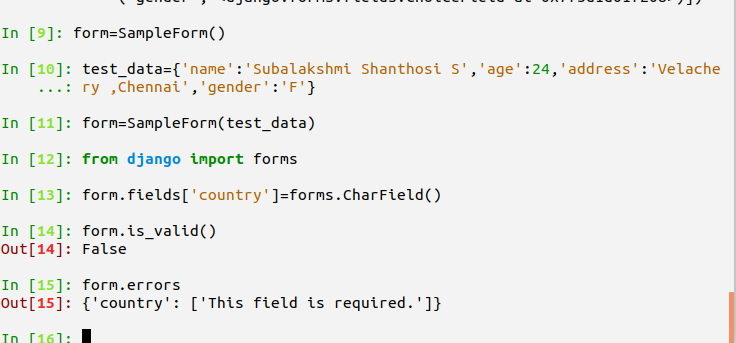
\includegraphics[scale=0.55]{project/includingFieldsForm.png}
\newpage
\subsection{Running Migration}

Migrations are Django's way of propagating changes you make to your models (adding a field, deleting a model,
etc.) into your database schema. They're designed to be mostly automatic, but you'll need to know when to make
migrations, when to run them, and the common problems you might run into.\\

There are several commands which you will use to interact with migrations and Django's handling of database schema:
\begin{enumerate}
	\item \textbf{migrate}, which is responsible for applying and unapplying migrations.
	\item \textbf{makemigrations}, which is responsible for creating new migrations based on the changes you have made to your models.
	\item \textbf{sqlmigrate}, which displays the SQL statements for a migration.
	\item \textbf{showmigrations}, which lists a project's migrations and their status.
\end{enumerate}
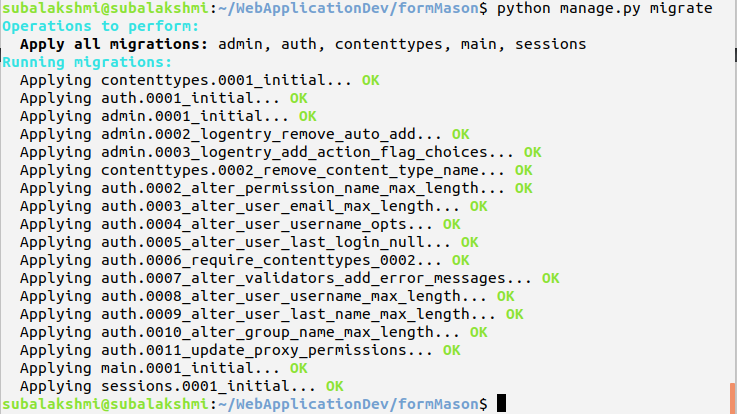
\includegraphics[scale=0.55]{project/migrationRunning.png}\\

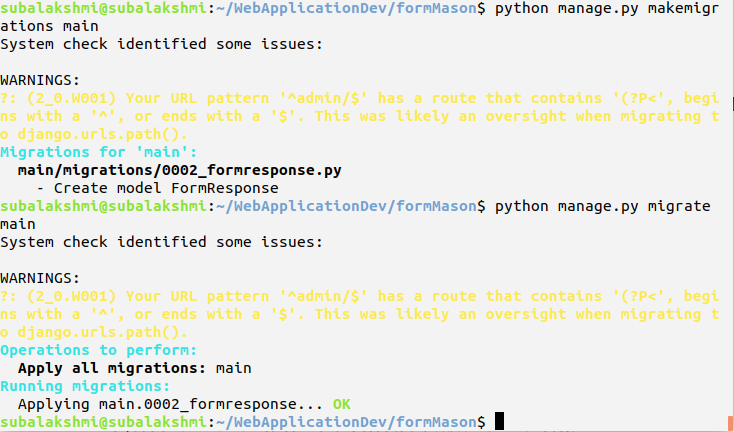
\includegraphics[scale=0.55]{project/savingRespMigration.png}
\subsection{Using created Model}
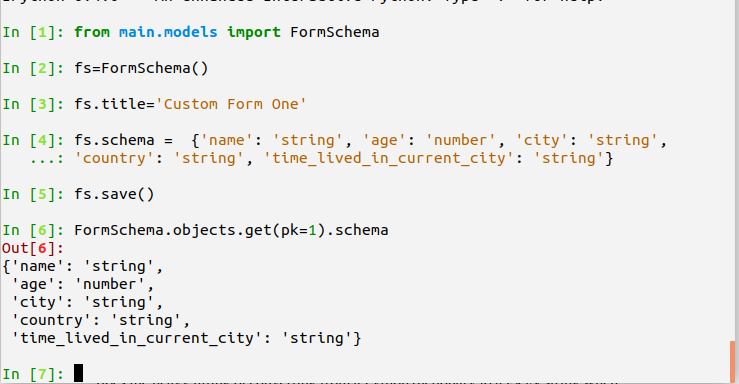
\includegraphics[scale=0.45]{project/formSchemaDefn.png}
